\chapter{线缺陷}
    \section{位错概念的引入}
        \subsection{实际晶体的滑移特征}
            在早期对金属材料的范性形变\index{范性形变}的研究中发现:
            \begin{itemize}
                \item[1] 单晶体发生范性形变时表面出现小台阶滑移线;
                \item[2] 晶体滑移总是沿着一定的密排晶面和密排方向,而且只有沿着这些面和方向的切应力达到一个临界值时,滑移才开始进行。
            \end{itemize}
            对与金属单晶来说,这个临界值在\SIrange{1}{10}{\MPa}。在这种情况下,人们引入晶体的理想模型来解决这个问题。

        \subsection{理想晶体的滑移}
            为了解释晶体的变形现象,人们提出了刚性滑移假设\index{刚性滑移假设}。
            假设滑移时滑移面两端的晶体为刚体,原子同步平移,设$T$为加载在晶体上的切应力,在缓慢变形中,该应力与变形相平衡。
            应力大小随滑移面两侧晶体相对位移量变化。

            由于晶体排列具有周期性,点阵对滑移的阻力也是周期性的,变形过程如\autoref{理想晶体变形示意图}所示,
            \begin{figure}[ht]
                \centering
                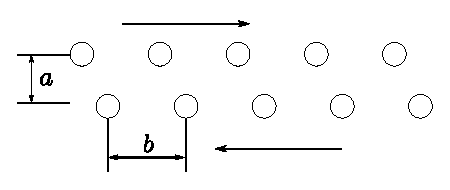
\includegraphics[width=0.7\textwidth]{fig/理想晶体变形示意图.eps}
                \caption{理想晶体变形示意图。}
                \label{理想晶体变形示意图}
            \end{figure}
            
            假定变形所受到的阻力为
            \begin{equation}
                \tau=\tau_m\sin{\left( \frac{2\pi x}{b} \right)}
            \end{equation}
            当发生的变形很小时,可以近似为
            \begin{equation}
                \tau=\tau_m{\left( \frac{2\pi x}{b} \right)},
            \end{equation}
            而且开始变形时,晶体处于弹性阶段,应当满足虎克定律,也就是
            \begin{equation}
                \tau=\mu\gamma=\mu\frac{x}{a},
            \end{equation}
            其中$\mu$为切变模量,$\gamma$为切应变,因此可以得到最大切应力为
            \begin{equation}
                \tau_m=\frac{\mu b}{2\pi a},
            \end{equation}
            由于本课程讨论的晶体绝大多数情况为简单立方晶系,可以认为$a=b$,所以最大切应变为
            \begin{equation}
                \tau_m=\frac{\mu}{2\pi}.
            \end{equation}

            然而理论切变强度$\frac{\mu}{2\pi}$与实际强度相比,实在太大。在使用更为合适的原子间作用力模型后,改变了正弦近似,
            最大切应变数值上降低为原来的$1/60$,但是这仍然比实际值高出了3到4个数量级。

            然而无论如何都提高应力模型的精确程度,最终结果的偏差仍然很大,因此是假设出现了问题。最终人们提出了位错模型,并且在
            实验中观察到了这一现象。
        
    \section{位错的结构}
        晶体中存在三种不同的位错类型,下面将分别描述。
            \subsection{刃型位错}
                考虑一个简单立方晶体,它在$(010)$面上沿$[100]$方向发生滑移,但是这个滑移是不均匀的。
                也就是从晶体的右侧向左传播。在某一时刻,滑移停止在晶体内部。于是在这个$(010)$面左右就可以划分出已滑移区域和未滑移区域,
                该面也就是两个区域的边界。晶体滑移的元过程是在一定的晶体学面上,沿一定的晶体学方向,晶体的上下两部分相对滑移一个或着多个
                点阵常数的距离。

                由此显然可见,已滑移的地区与未滑移的地区是一样的,上述滑移平面上下原子列是恢复对齐的,也就是说,这些地方恢复了理想晶体的长程
                有序性。所以除去\autoref{刃型位错形成示意图}中$\perp$的位置外,晶体的其他部分都是完整的。在这一区域内,晶体的完整周期性显然被
                破坏,所以这就是一个晶体缺陷,称为位错\index{位错}。
                \begin{figure}[ht]
                    \centering
                    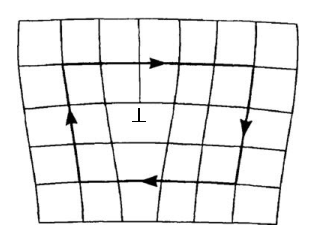
\includegraphics[width=0.45\textwidth]{fig/刃型位错示意图b.eps}
                    \caption{刃型位错形成示意图。}
                    \label{刃型位错形成示意图}
                \end{figure}

                关于位错最为简单的定义就是:位错是近完整晶体中的一个缺陷,是晶体中已滑移区和未滑移区的边界。
                
                这个边界更为严格的说,是分界区域的中心轴线,是平行于$[011]$方向的一条直线,其与滑移矢量$[100]$垂直,那么
                这个位错就称为刃型位错。

                上述中心轴线称为位错线\index{位错线},原理位错线的区域保持理想晶体的完整性;只有极为接近位错线的区域,也就是上述分界区域或
                过渡区域,晶体的点阵结构,或者原子的规则排列被破坏这一区域称为位错核心\index{位错!位错核心}。位错核心的半径与位错线的长度
                相比非常小,所以说,位错是晶体中的线性缺陷。

                对于刃型位错\index{位错!刃型位错},其与滑移矢量垂直,而\autoref{刃型位错形成示意图}中,$\perp$符号代表多余的一个半原子面,
                这个半原子面的边缘就是刃型位错的位错线,形状类似刀刃,因此称为刃位错\index{位错!刃位错}。
                因此刃型位错的形成也可以认为是一个半原子面中断与晶体内部,该边缘也就是一个刃型位错。

                在规定分割面的上下后,半原子面在割面上方的位错称为正刃型位错,反之则为负刃型位错,但是两者并没有本质上的区别。

                刃型位错有以下结构特点
                \begin{itemize}
                    \item[1] 位错周围有弹性畸变或非弹性畸变,上半部分晶体受压力,下部分受张力,中心为最大畸变,畸变局限在2或3个原子间距的管道内,总体为线缺陷;
                    \item[2] 位错线与滑移方向垂直;
                    \item[3] 上下晶体有一个相对位移$\vec{b}$,称为伯格斯矢量或简称柏式矢量\index{柏式矢量}。
                \end{itemize}
            \subsection{螺型位错}
                仍然假定滑移面为$\left( 010 \right)$面,位错线仍然是沿$[001]$方向的直线,但是滑移方向变为$[001]$方向,
                即为与位错线平行的方向,仍然将晶体分为已滑移区、未滑移区以及中间的过渡地带。同样,整个晶体是近完整的,只有在位错核心区,晶体的点阵
                结构才遭到破坏。
                
                也就是说,这也是一个二维缺陷,但是原子排列方式与刃型位错却不相同,不难得出,对与位错线垂直的原子面
                在位错不存在时,是一组彼此平行分立的平面,当此位错存在时,他们则变成一个连续的螺旋面。
                若绕此位错线以左手螺旋正向环行一周,即从一个面上升到相邻的另一个原子面,由于这个形质,这种位错称为螺型位错\index{位错!螺位错}。
                
                \begin{figure}[ht]
                    \centering
                    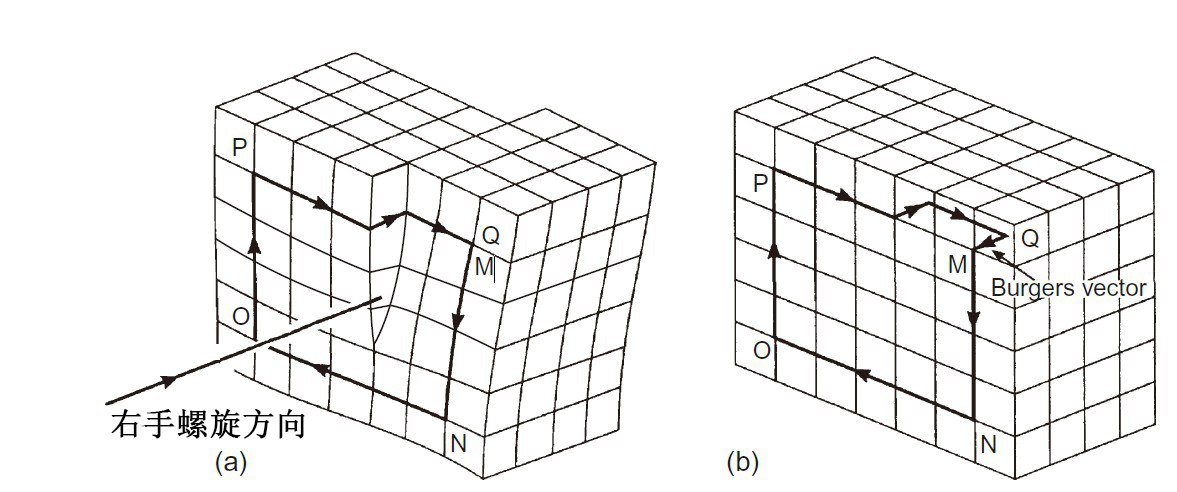
\includegraphics[width=0.7\textwidth]{fig/螺型位错示意图.jpg}
                    \caption{左螺型位错示意图,(a)螺型位错的左手螺旋回路,(b)为相同回路在理想晶体中的绕行状况。}
                    \label{螺型位错示意图}
                \end{figure}

                在规定位错线正方向后,若绕位错线以右手螺旋方向绕行一周后,可以上升一个原子面的位错为右螺型位错,
                若绕位错线以左手螺旋方向绕行一周后,可以上升一个原子面的位错为左螺型位错,如\autoref{螺型位错示意图}。
                左螺型位错和右螺型位错的滑移矢量方向也是相反的。

                在含有螺型位错的晶体中,原子面排布如\autoref{右螺型位错原子面排布}所示。晶体不再是刃型位错的附加半原子面,而是变成了螺旋式的曲面。
                \begin{figure}[ht]
                    \centering
                    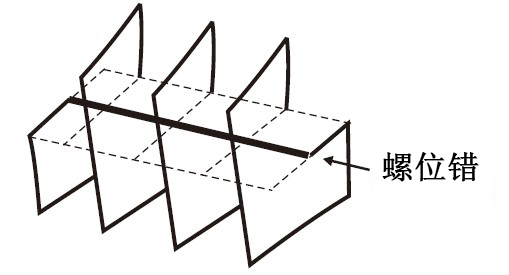
\includegraphics[width=0.5\textwidth]{fig/螺位错原子面排布.jpg}
                    \caption{右螺型位错原子面排布。}
                    \label{右螺型位错原子面排布}
                \end{figure}
            \subsection{混合型位错}
                然而一根直线位错可能既不与滑移矢量$\vec{b}$垂直,也不平行,而是成一个角度$\theta$,则这个位错既不是纯刃型位错也不是纯螺型位错,
                它可以看作是两个直线位错的叠加,分别为纯刃型和纯螺型的位错,两者的滑移矢量大小为
                \begin{align}
                    \vec{b}_1&=\vec{b}\sin\theta,\\
                    \vec{b}_2&=\vec{b}\cos\theta.
                \end{align}
                这个直线位错称为混合位错\index{位错!混合位错}。组成混合位错的两个分量为刃型分量和螺型分量。

                对上述情况加以推广,假设滑移矢量为$\vec{b}$,已滑移区域为\autoref{混合型位错的滑移示意}中的阴影部分,而位错线为图中红色线,从垂直与滑移面的方向看去,上下两个原子
                面之间的原子排布应该为\autoref{混合型位错的原子排列示意图}所示。
                \begin{figure}[ht]
                    \centering
                    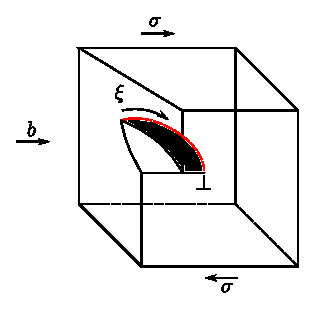
\includegraphics[width=0.5\textwidth]{fig/混合型位错的滑移示意.eps}
                    \caption{混合型位错的滑移示意。}
                    \label{混合型位错的滑移示意}
                \end{figure}
                
                \begin{figure}[ht]
                    \centering
                    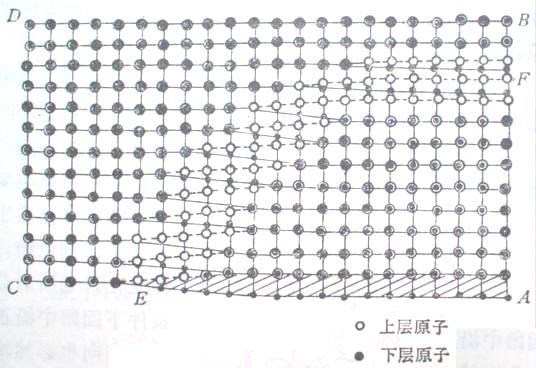
\includegraphics[width=0.5\textwidth]{fig/混合型位错的原子排列示意图.jpg}
                    \caption{混合型位错的原子排列示意图。}
                    \label{混合型位错的原子排列示意图}
                \end{figure}
                从\autoref{混合型位错的原子排列示意图}可以看出,这个位错有一段是纯螺型位错,另一端是纯刃型位错,由于位错线是连续的\footnote{这一点需要会证明。}
                从晶体的一个表面延伸到另一个表面,中间弯曲的一端既不是螺型位错也不是刃型位错,而是同时具有螺型和刃型位错的特征。
                这一小段也可以看作是许多方向近连续变化的小直线段所组成,每一小段都是混合型位错,各有一个螺型分量和刃型分量。
            \subsection{小结}
                依照以上定义,位错是晶体中滑移面上两个区域(即已滑移区域和未滑移区域)之间的分界,那么它就应该具有两个重要的性质:
                \begin{itemize}
                    \item[1] 因为晶体的滑移矢量是一个恒定矢量,等于一个或多个最小点阵平移矢量,所以对于一条位错线的各个部分,滑移矢量均相等;
                    \item[2] 无论位错线形状如何,总之位错线绝不可能终止于晶体的内部,位错线只能从晶体的一个表面延伸到另一个表面,或是在晶体中形成一个封闭的环。
                \end{itemize}
        \section{位错的普遍定义与伯格斯矢量}\label{section:位错的普遍定义与伯格斯矢量}
            \subsection{位错的普遍定义}
                在直观的基础上对位错的几何性质有一定的了解以后,我们这里可以对位错作出更为普遍的定义。

                假设晶体沿任意面$S$剖开,将$S$面的两边$S_1$以及$S_2$作一刚性的相对位移$\vec{b}$,$\vec{b}$可以是
                晶体中任意的电子平移矢量\footnote{$\vec{b}$不是点阵矢量的情形将在以后做出讨论。},经过这样的操作以后,
                如果$\vec{b}$与$S$面不平行,有些地方将产生原子位置重叠或者是空隙。去掉重叠的原子,空隙按照晶格排列填补,
                这样$S$面不会有任何改变,但是晶体中出现相对位移和未相对位移区域的分界线,也就是$S$面的周界。在分界线上原子错排的情况就是
                位错线\index{位错线},$\vec{b}$为伯格斯矢量或柏式矢量\index{柏式矢量},其为位错特征的标志,数值大小为$b$,
                称为位错的强度\index{位错!强度}。

                晶体中任意的位错都可以按照上面操作来形成, 但是汽油有一些需要注意的地方:
                \begin{itemize}
                    \item[1] 上述的想象操作不仅是用来说明位错的特征,也模拟了晶体产生位错的实际过程,关于位错生成的过程将以后讨论;
                    \item[2] 对于同一根位错线,可以有不同的$S$面,只要柏式矢量相图,形成的就是相同的位错,因此决定位错特征的是伯格斯矢量,而不是$S$面的具体位置,可以选以位错为边界的任意面作为上述操作的$S$面,比如沿$z$轴的刃型位错,选取$xoz$面和$yoz$面的结果是一致的;
                    \item[3] 实际上,从已经做过相对位移的区域到未作相对位移的区域间的过渡不可能是突变的,否则将产生无法填补的裂缝,因此$S$面两侧的刚性位移在边界是不再适用的,准确到说,位错不是一根线,而是有一定宽度$w$的区域,在这个区域内,$b$从中心的最大值下降到边界的零,只是由于宽度比长度小得多,所以可以近似为一根线。
                \end{itemize}
    
                \subsection{柏式矢量的定义}
                    $\vec{b}$矢量称为柏式矢量,它是位错线特征的标志,位错的强度为$b$,而方向的确定常使用伯格斯回路法和Frank惯例法。
                    \subsubsection{伯格斯回路法}
                        实现选取有位错的实际晶体,从好区中任意原子出发,微扰位错作一个闭合回路,回路每一步都连接相邻的同类原子,并且始终走在晶体的好区,这个回路称为伯格斯回路\index{伯格斯回路}。
                        然后在完整晶体中作一个对应的回路,即在相同方向走相同步数,结果发现这个回路无法闭合。终点到起点的矢量$\vec{b}$为柏式矢量\index{柏式矢量},回路
                        的方向与位错线方向成右手螺旋的方向为正方向。

                        假设晶体中三个基矢量$\vec{a}_0$,$\vec{b}_0$,$\vec{c}_0$,整个晶体的矢量都可以使用这三个矢量表示。
                        在理想晶体中,绕行晶体一周后必然有
                        \begin{equation}
                            \sum_{a}n_a\vec{a}_0+\sum_{c}n_b\vec{b}_0+\sum_{c}n_c\vec{c}_0=0\label{完整晶体的绕行结果},
                        \end{equation}
                        其中$n$为整数。

                        假如晶体不是完善的而是含有点缺陷,\autoref{完整晶体的绕行结果}仍然成立,但是基矢量在不同地方的长度有弹性范围内的差异,
                        这是因为点缺陷附近有弹性畸变,离开点缺陷稍远的地方,弹性畸变相应减少。

                        加入这个封闭回路本身经过的地方都是良好的,但是回路包围的区域中含有一个位错$\vec{b}$,回路的方向与位错的方向构成右手螺旋关系,对这个回路,\autoref{完整晶体的绕行结果}变为
                        \begin{equation}
                            \sum_{a}n_a\vec{a}_0+\sum_{c}n_b\vec{b}_0+\sum_{c}n_c\vec{c}_0=-\vec{b},                            
                        \end{equation}

                    \subsubsection{Frank惯例法}
                        Frank惯例法\index{Frank惯例法}需要线确定位错线的正向,割面及割面法线的正向,按照右手螺旋定则,四个手指顺位错线垂直防御割面上,大拇指指向正半晶体也就是法线方向,规定$\vec{b}$为
                        负半晶体相对与正半晶体的移动方向。

                        在确定$\vec{b}$后,如果位错线与$\vec{b}$平行,则为螺旋位错,方向相同为正,反向为负;如果$\vec{b}$与位错线垂直,
                        则为刃型位错,对于刃型位错的方向,需要使用半原子面右手法,如\autoref{刃型位错的半原子面右手法则}所示。
                        \begin{figure}[ht]
                            \centering
                            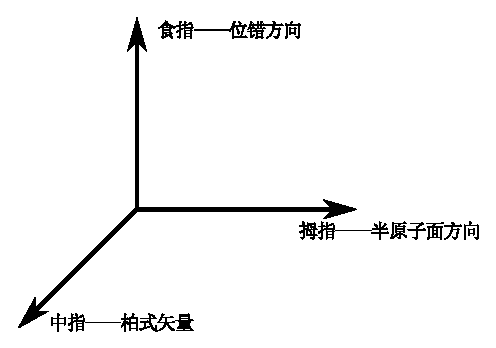
\includegraphics[scale=1]{fig/刃型位错的半原子面右手法则.eps}
                            \caption{刃型位错的半原子面右手法则。}
                            \label{刃型位错的半原子面右手法则}
                        \end{figure}
                \subsection{柏式矢量守恒定律}
                        利用柏式回路的概念即可论证伯格斯矢量的守恒定律:
                        \begin{enumerate}
                            \item[1] 一个位错线不可能中止于晶体内部,它必然构成闭合1的圈或终止于晶体表面,沿一根不分岔的位错线的伯格斯矢量是守恒的,具有相图的大小和方向。
                            \item[2] 如果数根位错线相较于一点,此点称为位错的节点\index{节点},朝向节点的各位错线柏式矢量的总和等于流出各节点位错线伯格斯矢量矢量的总和,如果所有的位错线方向都是从节点出发,则上述关系可以写作各分支柏式矢量的总和为零,即$\sum b=0$;
                            \item[3] 柏式回路有如下特点:
                            \begin{enumerate}
                                \item[1)] 一根位错线只有一个柏式矢量;
                                \item[2)] 位错线不能在晶体内部中断,因而它们只能或者终止在晶体表面,或者形成封闭环,或者与其它位错相联;
                                \item[3)] 当位错与其它位错相联时,指向结点的位错柏氏矢量和与离开节点位错的柏氏矢量和相等,若均指向一个节点,有$\sum b=0$。
                            \end{enumerate} 
                        \end{enumerate}
        
        \section{位错应力场}
            根据\autoref{section:位错的普遍定义与伯格斯矢量},位错是一个线缺陷,其最大畸变分布在以位错线为轴心的管道区域内,管道的直径为2到3个原子间距。
            同时位错的畸变与距离位错线的距离成反比,距离越远的区域,畸变也越小。
            但是由于位错造成的畸变遍布整个晶体,所以伴随这些畸变也造成了晶体各原子之间的位置发生变化,偏离了
            原来的平衡位置,相互之间产生了内应力的作用,应力和应变的乘积即是造成系统能量上升的原因,因此需要定量地分析位错在晶体中所引起的畸变
            和能量。

            为了方便研究,一般把晶体分成两个区域
            \begin{itemize}
                \item[1] 位错中心,由于这个区域畸变严重,必须要考虑晶体结构和原子间相互作用,才能分析应力场和相应的能量;
                \item[2] 远离位错中心的区域,这一部分畸变相对较小,因此可以使用线弹性理论处理。
            \end{itemize}
            
            如\autoref{螺型位错的连续介质模型}所示,沿$z$方向位错线取一个圆柱体,由于中心位置畸变能过大,将其中心挖去,挖掉的区域半径为$r_0$。
            圆柱体沿$z$方向错开一个原子间距$b$,也就是晶体中出现了一个螺位错。假设所研究的点距离中心为$r$,则在绕行一周后,弹性畸变为$b$,平均单位周长变形为
            \begin{equation}
                \varepsilon=\frac{b}{2\pi r}.
            \end{equation}

            \begin{figure}[ht]
                \centering
                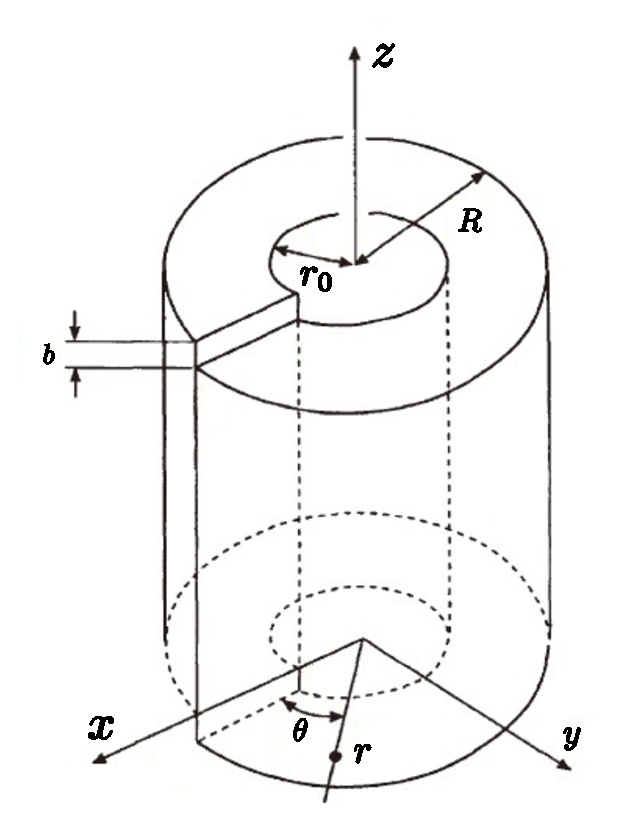
\includegraphics[scale=0.5]{fig/螺型位错的连续介质模型.eps}
                \caption{螺型位错的连续介质模型。}
                \label{螺型位错的连续介质模型}
            \end{figure}

            在柱坐标系中,平均单位周长变形为
            \begin{equation}
                \gamma_{z\theta}=\frac{b}{2\pi r},
            \end{equation}
            由于是弹性变形,代入到胡克定律中,有
            \begin{equation}
                \tau_{z\theta}=\mu\gamma=\frac{\mu b}{2\pi r}, r>r_0.
            \end{equation}
            其中$\mu$为切变模量。

            在直角坐标系中,可以得出
            \begin{align}
                \tau_{xz}&=-\frac{\mu b}{2\pi}\frac{y}{x^2+y^2},\\
                \tau_{yz}&=\frac{\mu b}{2\pi}\frac{x}{x^2+y^2},
            \end{align}
            由此可以看出,
            \begin{itemize}
                \item[1] 在晶体中,只要有位错就有应力场,而不管此晶体是否有外加应力,外加应力与位错产生的应力场无关;
                \item[2] 不同$r$都有应力场,也就是说,位错应力是一个长程应力场,遍布于整个晶体的应力场;
                \item[3] 伴随$r$增大,$\tau$减小,因此距离位错中心越远的地方,应力也就越小;
                \item[4] 根据公式的结果,$r$趋于0,$\tau$为无限大,因此上述公式不再适用于这种情况,这与挖掉位错核心这一方法相符。
            \end{itemize}
            关于位错的应力场的分布则主要是弹性力学的内容,这里不再关注。

            \subsection{刃型位错的应力场}
                假设晶体没有边界,体积无限大,刃位错的位错线沿$z$方向,符号为正,如\autoref{刃型位错的连续介质模型}所示,则
                \begin{figure}[ht]
                    \centering
                    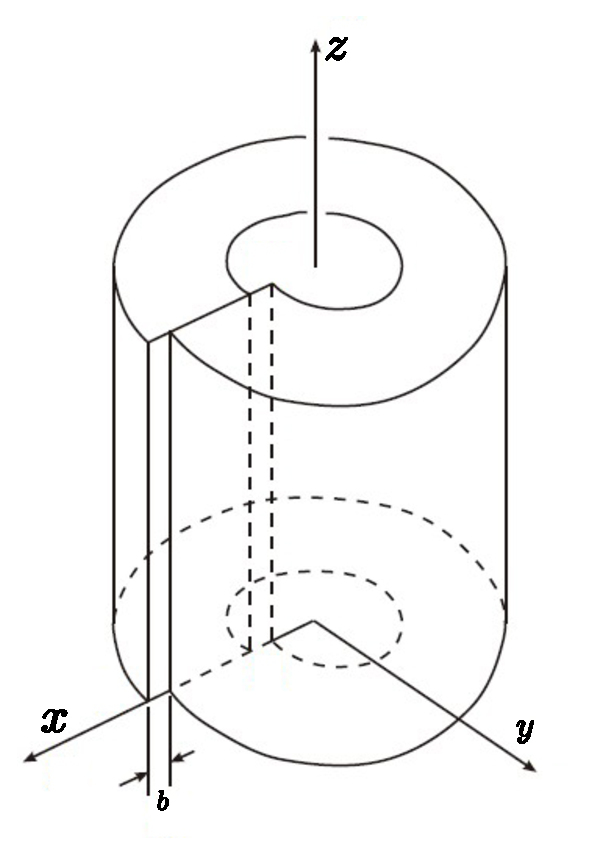
\includegraphics[scale=0.5]{fig/刃型位错模型.eps}
                    \caption{刃型位错的连续介质模型。}
                    \label{刃型位错的连续介质模型}
                \end{figure}
                应力场的主应力及分量为:
                \begin{align} 
                    \sigma_{x x} &=-\frac{\mu b}{2 \pi(1-v)} \frac{y\left(3 x^{2}+y^{2}\right)}{\left(x^{2}+y^{2}\right)^{2}}, \\ 
                    \sigma_{y y} &=\frac{\mu b}{2 \pi(1-v)} \frac{y\left(x^{2}+y^{2}\right)}{\left(x^{2}+y^{2}\right)^{2}}, \\
                    \tau_{x y} &=\frac{\mu b}{2 \pi(1-v)} \frac{x\left(x^{2}-y^{2}\right)}{\left(x^{2}+y^{2}\right)^{2}}, \\
                    \sigma_{z z} &=v\left(\sigma_{x x}+\sigma_{y y}\right), \\
                    \tau_{x z} &=\tau_{y z}=0 .
                \end{align}
                其中$v$为泊松比,改用柱坐标系后上述关系变为
                \begin{align}
                    \sigma_{r r}&=\sigma_{\theta \theta}=-\frac{\mu b}{2 \pi(1-v)} \frac{\sin \theta}{r}, \\ 
                    \sigma_{r \theta}&=\frac{\mu b}{2 \pi(1-v)} \frac{\cos \theta}{r}, \\ 
                    \sigma_{z z}&=v\left(\sigma_{r r}+\sigma_{\theta \theta}\right).
                \end{align}
                从刃型位错应力场的表达式可以发现,刃型位错有以下特点
                \begin{enumerate}
                    \item[1] 应力场与$z$方向无关,是平面型的;
                    \item[2] 正应力场关于$yoz$面和$y$轴对称,而且$|\sigma_{xx}|>|\sigma_{yy}|$,
                    \begin{enumerate}
                        \item[a] 当$y>0$也就是上半晶体,$\sigma_{xx}<0$,受压应力,
                        \item[b] 当$y<0$也就是下半晶体,$\sigma_{xx}>0$,受张应力;
                    \end{enumerate} 
                    \item[3] 应力大小与$b$大小有关,而且当$r$增大,应力下降,这与简化分析得到的结果一致;
                    \item[4] $y=0$时,$xoz$面也就是位错的滑移面上有
                            \begin{align}
                                \sigma_{xx}&=\sigma_{yy}=0,\\
                                \tau_{xy}&=\tau_{yx}.
                            \end{align} 
                            也就是切应力在滑移面上有最大值。
                \end{enumerate}
            \subsection{螺型位错的应力场}
                在直角坐标系下,\autoref{螺型位错的连续介质模型}的应力场表达形式为
                \begin{align} 
                    \tau_{x z} &=-\frac{\mu b}{2 \pi} \frac{y}{x^{2}+y^{2}}, \\
                    \tau_{y z} &=\frac{\mu b}{2 \pi} \frac{x}{x^{2}+y^{2}}. 
                \end{align}
                在柱坐标系下,有
                \begin{equation}
                    \tau_{\theta z}=\tau_{z\theta}=\frac{\mu b}{2\pi r},
                \end{equation}
                而其他的应力分量均为0。而螺型位错的应力场的特点为
                \begin{itemize}
                    \item[1]  螺型位错的应力场只有切应力分量,没有正应力分量,所有的正应力分量均等于0。
                    \item[2] 应力大小和$b$有关,并且随着$r$越大、应力越小;
                    \item[3] 应力是轴对称的,与$θ$ 无关。
                \end{itemize}
            \subsection{混合位错的应力场}
                混合型位错可以采用将柏氏矢量分解的办法进行求解,我们可以发现,位错线平
                行的螺型位错由于没有正应力分量,因此其正应力分量只要采用刃型位错的正应力分
                量即可。
                
                同时刃型位错的切应力分量只有$\tau_{xy}$分量,而螺型位错的切应力分量为$\tau_{xz}$和$\tau_{yz}$,
                因此没有相互重叠的应力分量,可以进行叠加。因此可以总结为如下的特点:
                \begin{itemize}
                    \item[1] 螺型和刃型没有重叠分量;
                    \item[2] 应力场互不影响;
                    \item[3] 因此混合型可以分解为螺型与刃型分量分别计算并叠加。
                \end{itemize}
        \section{位错的应变能}
        \section{位错的线张力}
        \section{位错核心}
        \section{位错的受力与运动}
        \section{位错与晶体缺陷间的相互作用}
        \section{位错的增殖}
        \section{实际晶体中的位错}
        